\chapter{Конструкторская часть}

\section{Описание алгоритмов}

Алгоритмы поиска (рисунки \ref{fig:lin} и \ref{fig:bin}) в массиве получают на вход массив arr, размер массива n и значение value.

\begin{figure}[h!]
	\centering
	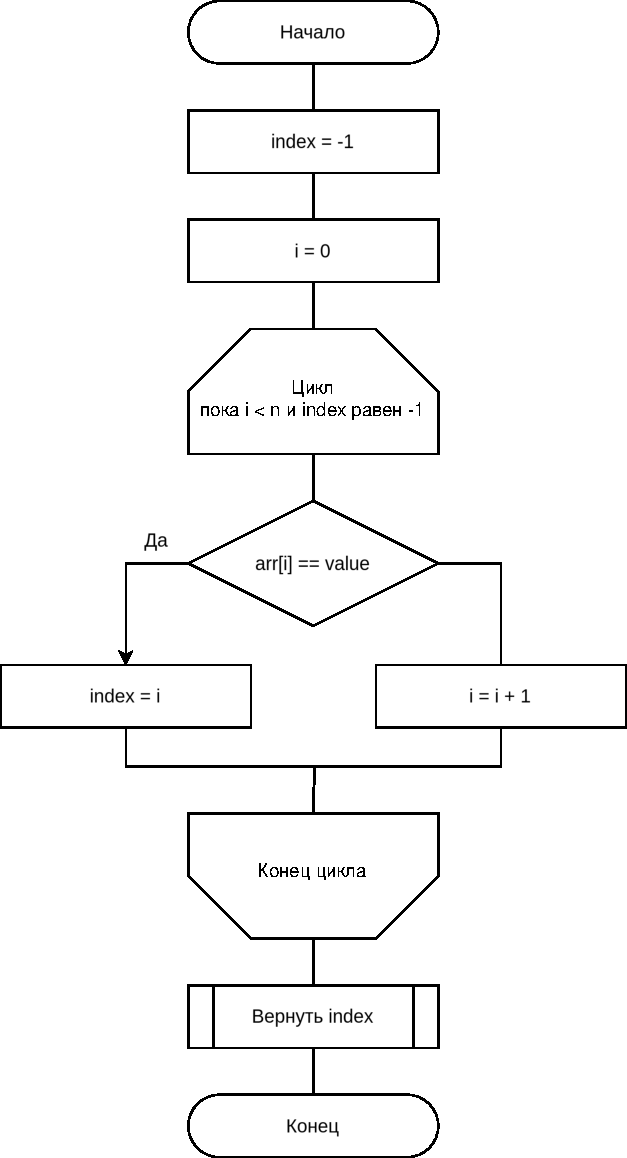
\includegraphics[width=0.6\textwidth]{tex_parts/linear.pdf}
	\caption{\label{fig:lin}Схема алгоритма линейного поиска в массиве}
\end{figure}

\begin{figure}[h!]
	\centering
	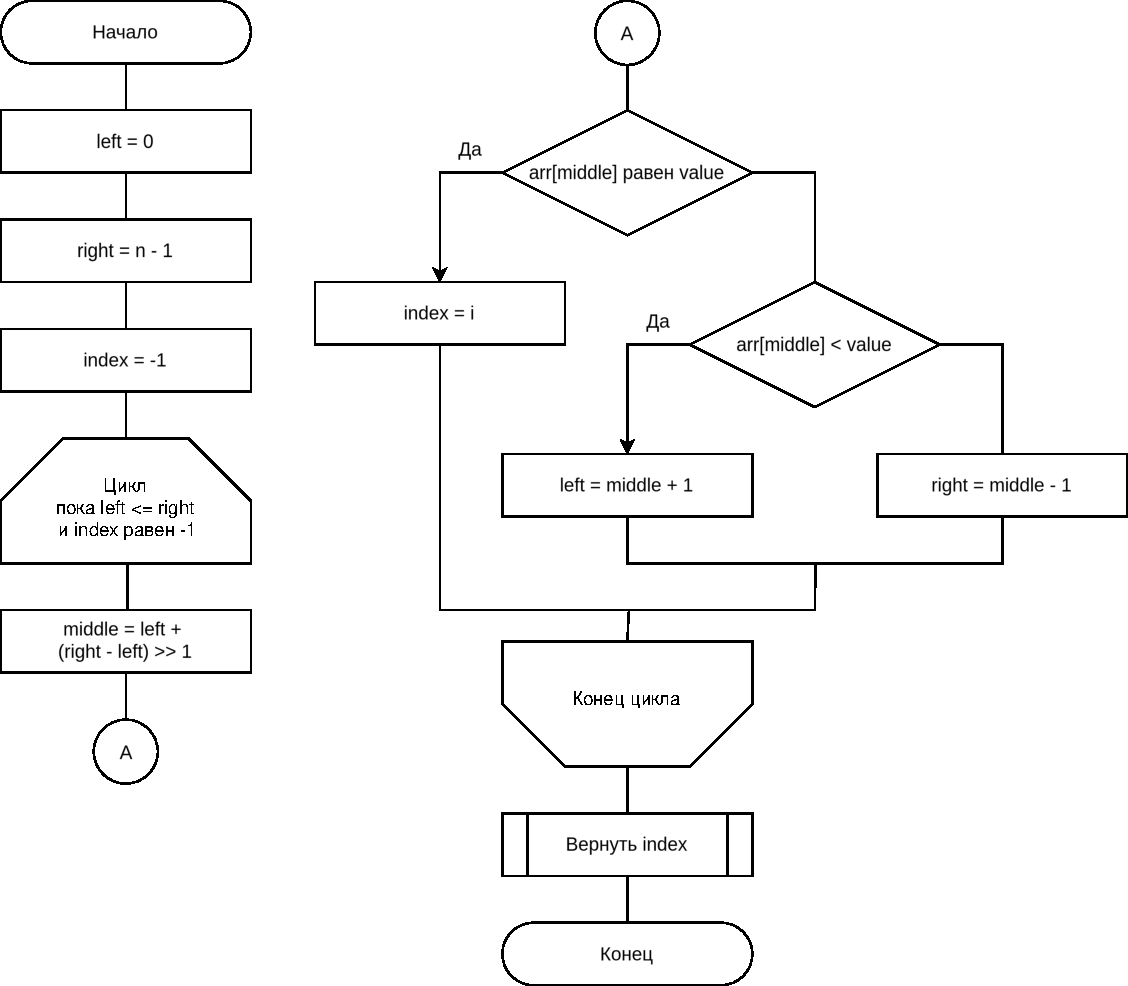
\includegraphics[width=0.6\textwidth]{tex_parts/binary.pdf}
	\caption{\label{fig:bin}Схема алгоритма бинарного поиска в массиве}
\end{figure}

Алгоритм пирамидальной сортировки (рисунок \ref{fig:sort}) получает на вход массив arr и размер массива n. В нём swap -- функция, меняющая местами переменные, а heapify -- функция восстановления свойства кучи.

\begin{figure}[h!]
	\centering
	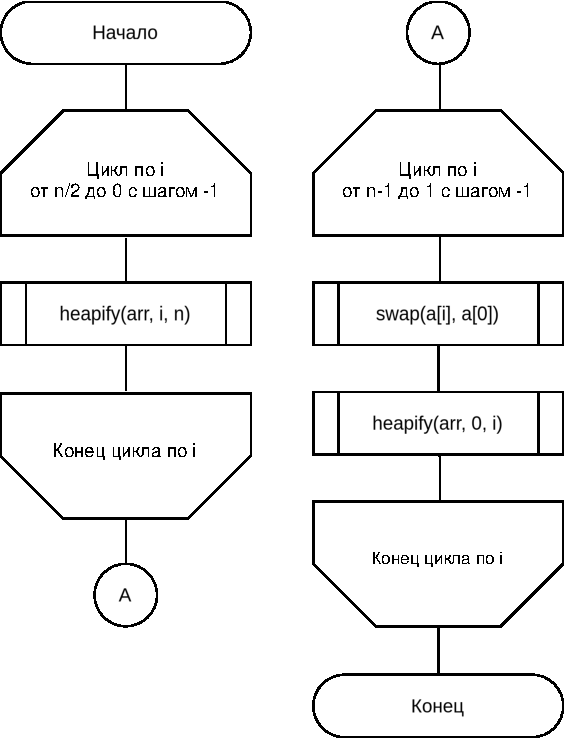
\includegraphics[width=0.5\textwidth]{tex_parts/sort.pdf}
	\caption{\label{fig:sort}Схема алгоритма пирамидальной сортировки}
\end{figure}

\clearpage

Алгоритм восстановления свойства кучи (рисунок \ref{fig:heap}) в вершине получает на вход массив arr, размер массива size и индекс index. В нём swap -- функция, меняющая местами переменные.

\begin{figure}[h!]
	\centering
	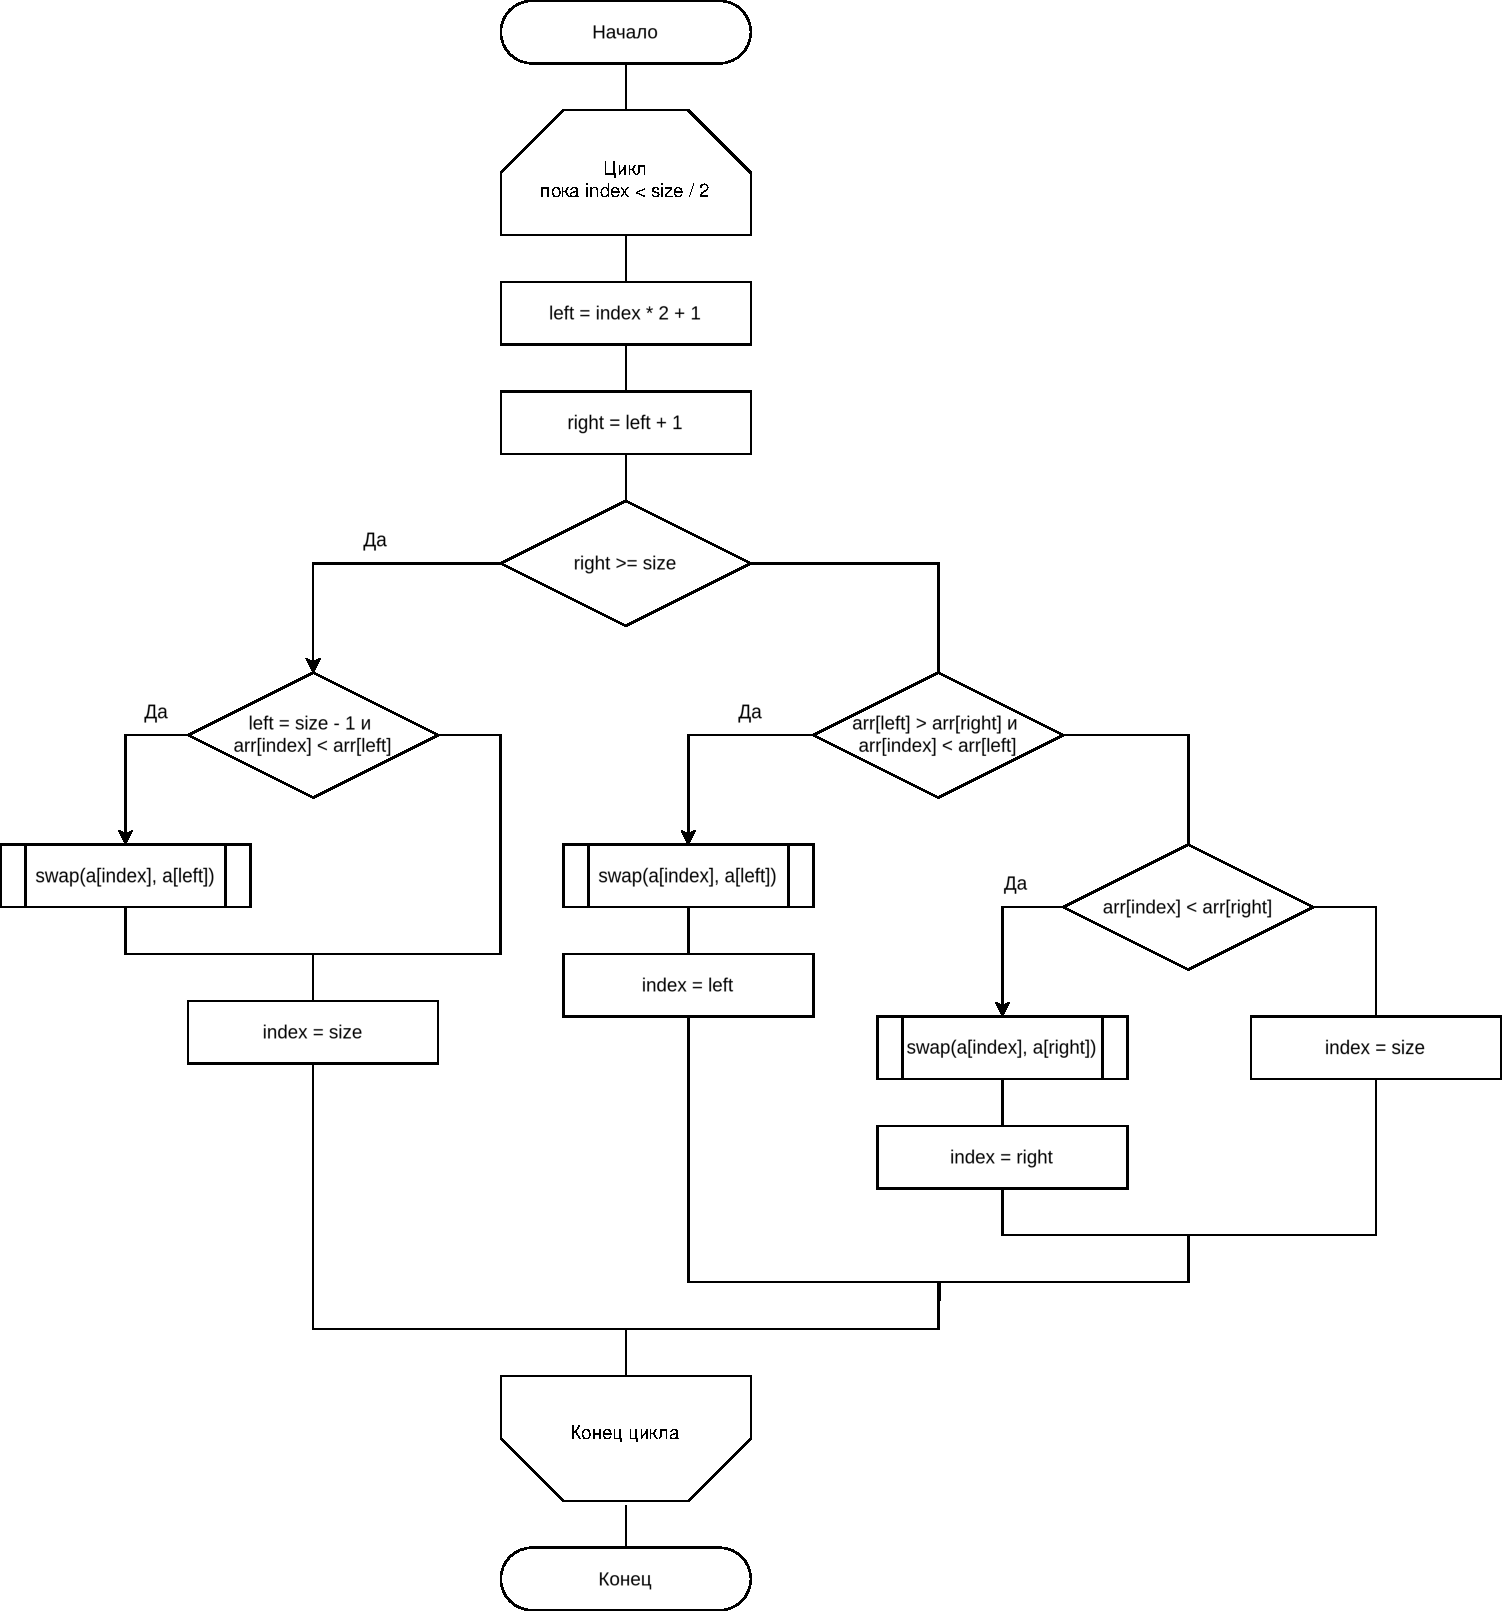
\includegraphics[width=0.8\textwidth]{tex_parts/heapify.pdf}
	\caption{\label{fig:heap}Схема алгоритма восстановления свойства кучи в вершине}
\end{figure}

\section{Выводы}

В данном разделе были построены схемы алгоритмов и выбраны структуры данных.

